%%% Einfaches Template für einen Abschlussbericht zum Berufspraktikum
%%% äöüÄÖÜß  <-- keine deutschen Umlaute hier? UTF-faehigen Editor verwenden!

%%% Magic Comments zum Setzen der korrekten Parameter in kompatiblen IDEs
% !TeX encoding = utf8
% !TeX program = pdflatex 
% !TeX spellcheck = de_DE
% !BIB program = biber

\RequirePackage[utf8]{inputenc} % bei Verw. von lualatex oder xelatex entfernen!
\RequirePackage{hgbpdfa}        % Erzeugt ein PDF/A-2b-konformes Dokument

\documentclass[internship,german,smartquotes,alphabetic]{hgbthesis}
% Zulässige Optionen in [..]: 
%    Typ der Arbeit: 'diploma', 'master' (default), 'bachelor', 'internship'
%		 Zusätzlich für ein Thesis-Exposé: 'proposal' (für 'bachelor' und 'master')
%    Hauptsprache: 'german' (default), 'english'
%    Option zur Umwandlung in typografische Anführungszeichen: 'smartquotes'
%    APA Zitierstil: 'apa'
%%%-----------------------------------------------------------------------------

\graphicspath{{images/}}  % Verzeichnis mit Bildern und Grafiken
\logofile{logo}           % Logo-Datei: images/logo.pdf (kein Logo: \logofile{})
\bibliography{references} % Biblatex-Literaturdatei (references.bib)

\usepackage{hyperref}
\usepackage[acronym]{glossaries}

\makeglossaries

\newacronym{jvm}{JVM}{Java Virtual Machine}
\newacronym{vt}{VT}{Virtual Thread}
\newacronym{pt}{PT}{Plattform Thread}
\newacronym{ot}{OT}{Betriebssystem Thread}
\newacronym{sts}{STS}{StructuredTaskScope}                          % makeglossaries main in der cmd ausführen
% \makeglossaries                           % makeglossaries muss dadurch nicht mehr in der cmd ausgeführt werden  


%%%-----------------------------------------------------------------------------
\begin{document}
%%%-----------------------------------------------------------------------------

%%%-----------------------------------------------------------------------------
% Angaben für die Titelei (Titelseite, Erklärung etc.)
%%%-----------------------------------------------------------------------------

% \title{Endbericht zum Berufspraktikum bei Mogulovich International}
% \author{Alex A.\ Schlaumeier}

% \programtype{Fachhochschul-Bachelorstudiengang}

% \programname{Medientechnik und -design}
% \placeofstudy{Hagenberg}

% \dateofsubmission{2024}{06}{25}
% \advisor{Pjotr I.~Czar, M.A.}
% \companyName{%
%    Mogulovich International Media GmbH\\
%    Online Division\\
%    Hubertusgasse 3a, 1020 Wien
% }
% \companyUrl{www.mogul.at}
\pagenumbering{alph}                    % damit die Titelseite mit 'a' beginnt und links wieder richtig funktionieren
% 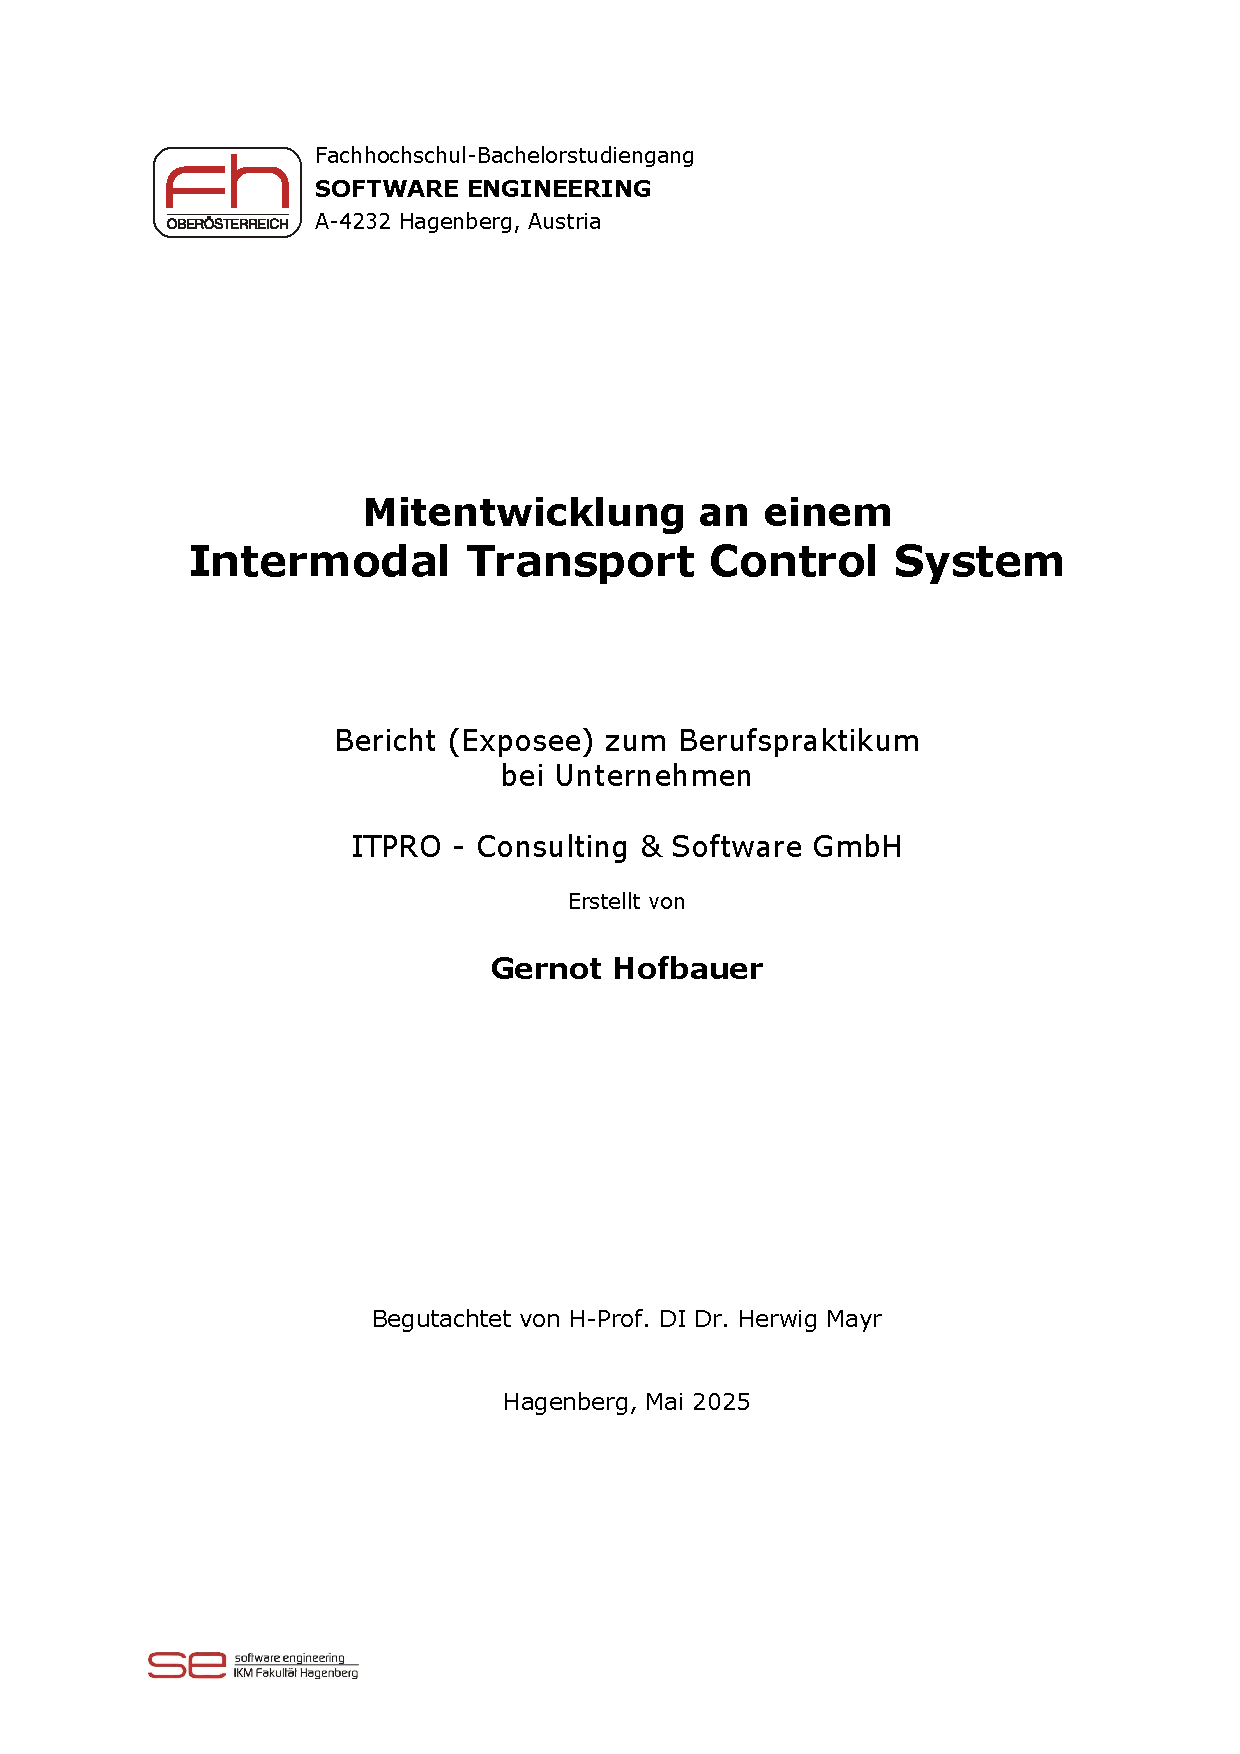
\includepdf[pages=-]{Titelblatt.pdf}
%%%-----------------------------------------------------------------------------
\frontmatter                                       % Titelei (röm. Seitenzahlen)
%%%-----------------------------------------------------------------------------

% \maketitle
\tableofcontents
\printglossary[type=\acronymtype,title=Akronyme]

%%%-----------------------------------------------------------------------------

% \chapter{Kurzfassung}% Umfang der Kurzfassung: ca.\ 200 Worte.
Dieser Praktikumsbericht beschreibt die Arbeit des Praktikanten im Rahmen seines Praktikums bei der Firma ITCS GmbH. Der Schwerpunkt lag auf der Entwicklung
von Software für das ITCS-Management-System, das in der öffentlichen Verkehrsinfrastruktur eingesetzt wird. Das Herzstück dieser Software ist eine Webanwendung,
die es ermöglicht, Umläufe aus einzelnen Fahrten zu erstellen. Dabei sollten verschiedene benötigte Daten auf der darunterliegenden Datenbank generiert werden.
Außerdem sollten diese Umläufe auch automatisch auf Durchführbarkeit geprüft werden.
In diesem Praktikum wurde mit der Programmiersprache \emph{C\#} und dem \emph{.NET}-Framework gearbeitet. Der Datenbankzugriff erfolgte über die \emph{Entity Framework Core}-Bibliothek, 
die eine objektorientierte Abstraktionsebene für den Datenbankzugriff bereitstellt. Das Frontend wurde mit \emph{Blazor} entwickelt, einer modernen Webtechnologie, 
die es ermöglicht, interaktive Webanwendungen mit C\# zu erstellen. Durch die Verwendung von \emph{Blazor} konnte eine nahtlose Integration zwischen Frontend und Backend erreicht werden,
was die Entwicklung effizienter und flexibler machte.
Während der Implementierung diese Umlaufeditors musste auch teilweise das bestehende Datenmodell angepasst werden, um die neuen Anforderungen zu erfüllen. 
Da die Datenbank mit Daten aus anderen Systemen gefüllt wird, musste auch ein anderes, bestehendes Projekt, das für den Import und Export von Daten benutzt ist, angepasst werden.
Dabei musste darauf geachtet werden, dass die Daten weiterhin mit dem \emph{VDV-452}-Standard kompatibel bleiben, um die Interoperabilität mit anderen Systemen zu gewährleisten.

%%%-----------------------------------------------------------------------------
\mainmatter                             % Hauptteil (ab hier arab. Seitenzahlen)
%%%-----------------------------------------------------------------------------
\chapter{Einleitung}
\label{cha:Einleitung}

    Seit einigen Jahren Arbeitet Oracle an Möglichkeiten zur Verbesserung der Skalierbarkeit von Java-Anwendungen im Projekt "Loom".
    Der Hauptansatz dieses Vorhabens ist die Einführung von virtuellen Threads, die von der JVM verwaltet werden. 
    Diese Threads sind leichtgewichtiger als klassische Plattform Threads und können in größerer Anzahl erzeugt werden.
    So können bestimmte Anwendungen mit hoher Nebenläufigkeit zukünftig effizienter gestaltet werden. Diese Bachelorarbeit 
    beleuchtet diese Technologien und stellt die Neuerungen dem bereits Bekanntem gegenüber.

\section{Ziel der Arbeit}
\label{sec:Ziel}

    Das Ziel dieser Bachelorarbeit ist es, die grundlegenden Eigenschaften und Limitierungen des bestehenden Thread-Konzepts zu untersuchen und die Motivationen für die Neuerungen
    durch Projekt Loom zu verstehen. Ein Überblick über Projekt Loom und die damit verbundenen Technologien wird gegeben, wobei der Schwerpunkt auf Virtual Threads liegt. 
    Die Arbeit soll zeigen, wie und in welchen Fällen diese Neuerungen in der Praxis angewendet werden können und welche neuen Möglichkeiten sich dadurch ergeben. 
    Es wird auch verdeutlicht, welche bestehenden Probleme der parallelen Ausführung durch die neuen Technologien nicht gelöst werden können. 
    Durch Benchmarks sollen Laufzeit und Speicherverbrauch unter verschiedenen Umständen analysiert werden, um daraus Schlüsse zu ziehen, 
    in welchen Fällen die neuen Technologien verwendet werden sollten und in welchen nicht. Als konkretes Ergebnis wird eine Sammlung kleinerer Programme erstellt, 
    die die neuen Technologien in Projekt Loom demonstrieren und die Unterschiede zu den bisherigen Technologien aufzeigen.




\chapter{Design}\label{chap:design}

    Da wie bereits erwähnt, die Projekte \emph{"ITCS-Management"} und \emph{"ITCS"} bereits existierten, waren das grundlegende Design und die technische Architektur bereits vorgegeben.
    Dies umfasst sowohl Aspekte wie die Transaktionsverwaltung der Datenbank, als auch Elemente im Frontend, wie die Navigation zwischen den Seiten oder die Farbpalette.

\section{"ITCS-Management"}\label{sec:itcs-management-design}
    Im Projekt \emph{"ITCS-Management"} wurde eine Vielzahl an kleineren Aufgaben erledigt. Dabei handelte es sich um Blazor-Seiten, die meist nur Datenbank-Entitäten tabellarisch
    darstellen und beschränktes Editieren ermöglichen sollten. Im Bericht selbst wird auf diese Aufgaben, aufgrund ihrer repetitiven Natur, nicht weiter eingegangen. Fokussiert wird  
    auf die größte Aufgabe in diesem Projekt namens \emph{"Umlaufeditor"}. 
    Ein Umlauf stellt dabei eine Sequenz von Fahrten dar, die von einem einzelnen Fahrzeug in einem Durchgang durchgeführt wird. Die Fahrten werden von den meisten Kunden in anderen 
    Systemen erstellt und sind mit dem Import neuer Versionen in der Datenbank schon vorhanden. Die Umläufe hingegen werden nicht in anderen Systemen definiert und sollen deswegen
    mit diesem Editor erstellt und angepasst werden. 
    \begin{figure}[H]
        \centering
        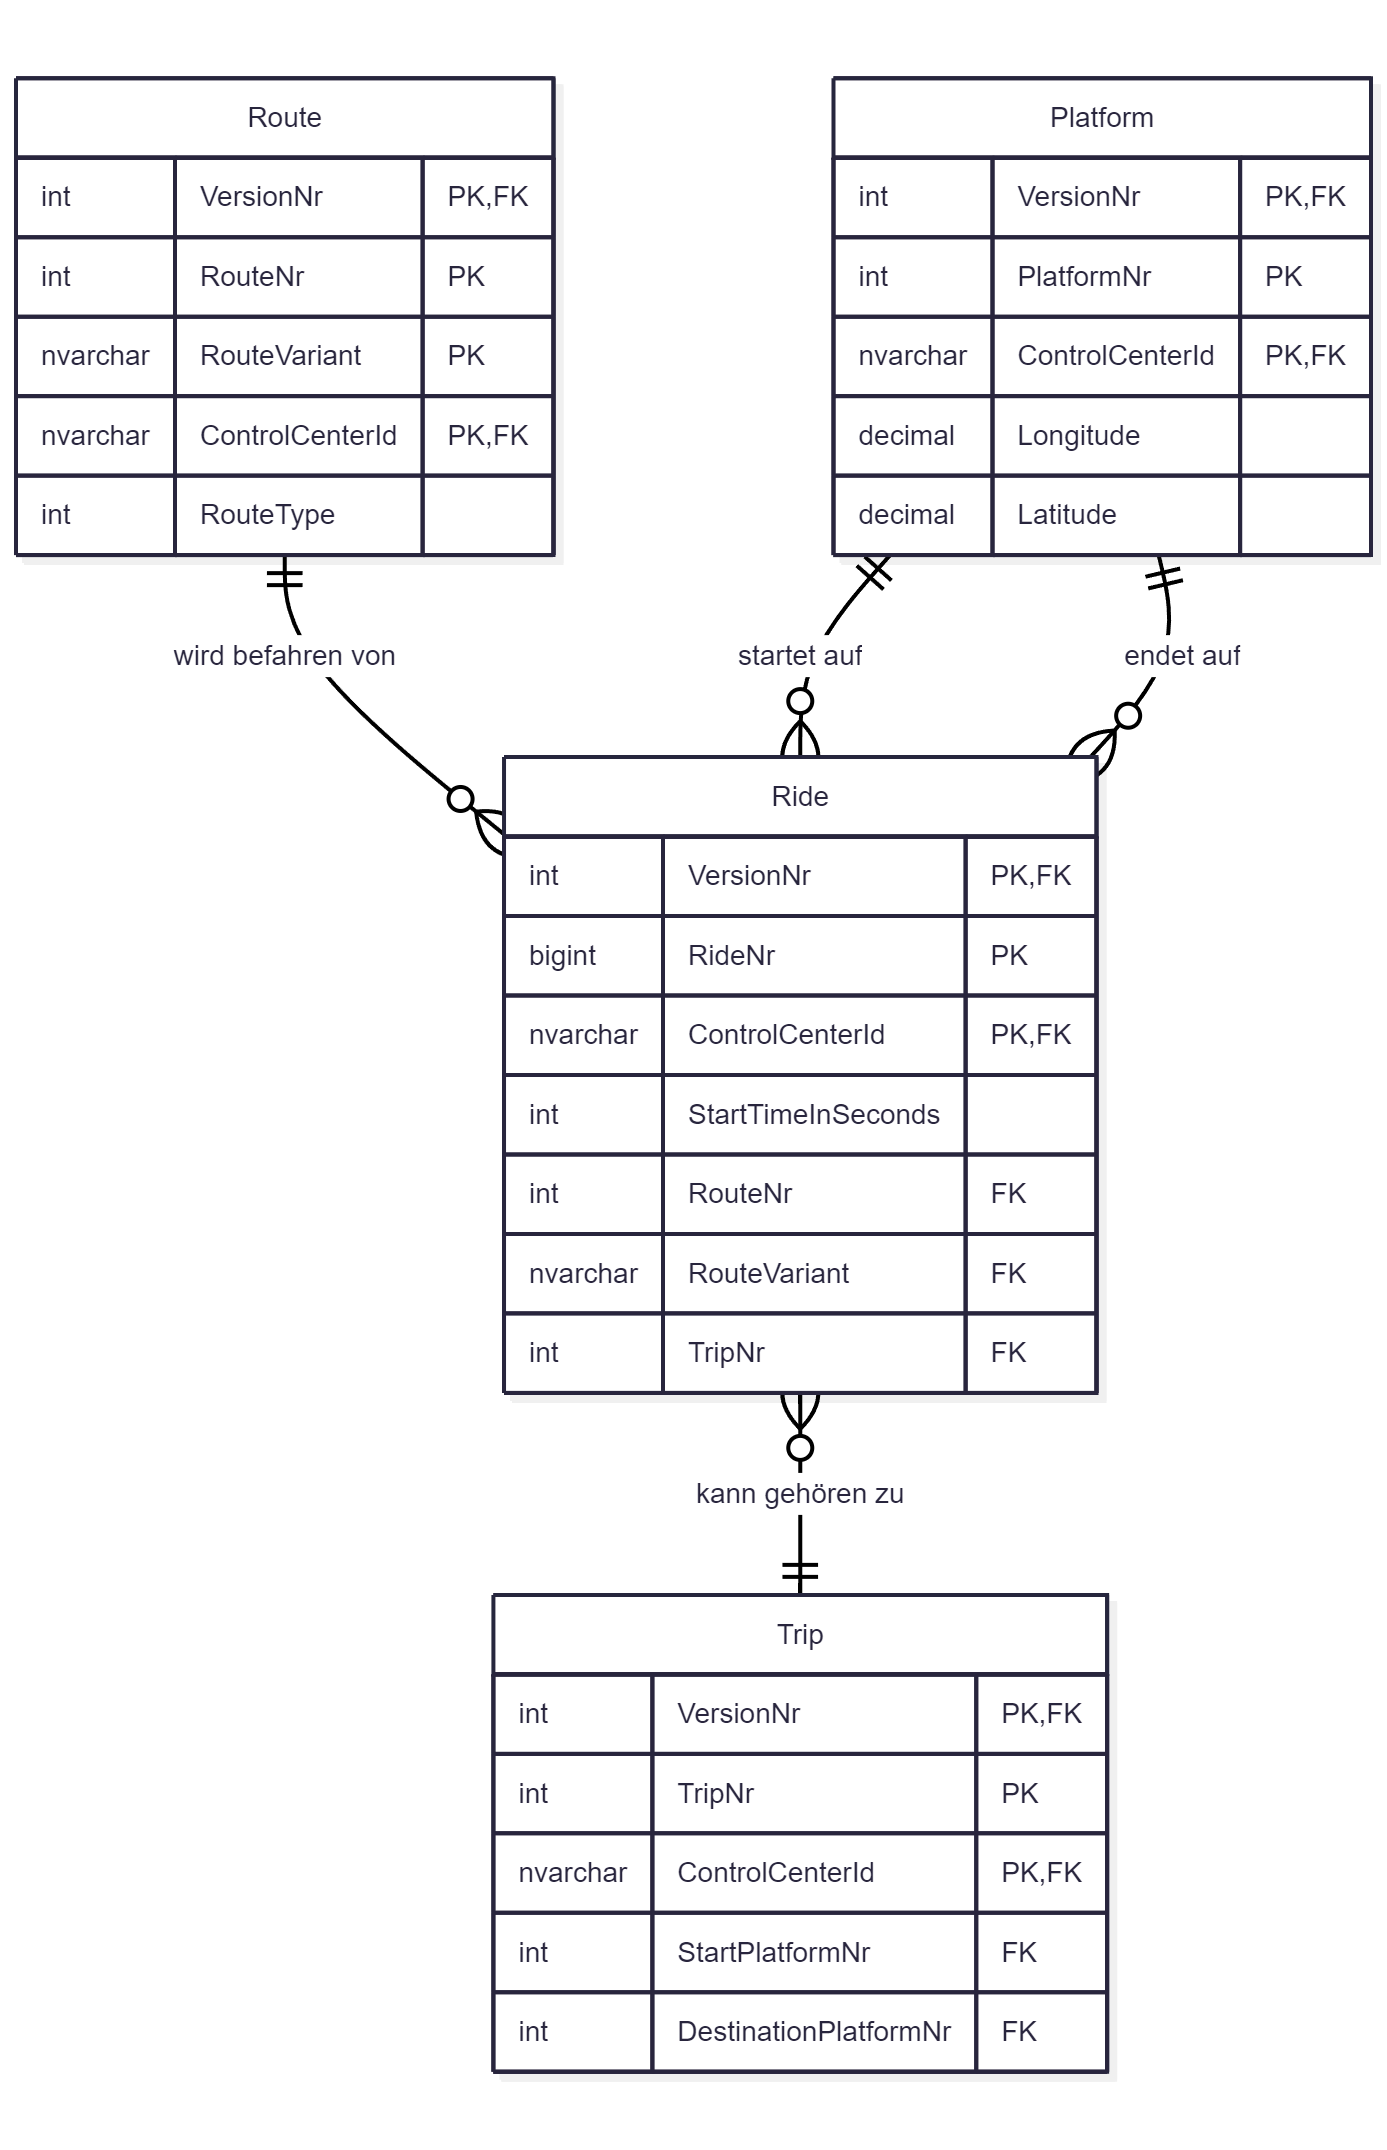
\includegraphics[width=0.8\textwidth]{transportation_system.png}
        \caption{Beziehungen von Umläufen und Fahrten}
        \label{fig:BeziehungenvonUmläufenundFahrten}
    \end{figure}

    Abbildung \ref{fig:BeziehungenvonUmläufenundFahrten} soll einen groben Überblick über das unmittelbar für diese Aufgabe benötigte Datenschema verschaffen. Für das Verständnis unwesentliche 
    Datenkomponenten und Beziehungen wurden weglassen. Die Entität "Route" ist in diesem Modell deswegen wichtig, da die Datenkomponente "RouteNr" die Art der Fahrt festlegt. Für Pausen oder nicht
    produktive
    Fahrten wird eine eigene Nummer vergeben. Zusätzlich ist bei jedem Umlauf ebenfalls jeweils eine Plattform-Entität (auch "Steig") als Start- und Endpunkt eingetragen. Dabei kann es sich bei den 
    Steigen um Sonderhaltepunkte wie beispielsweise Betriebshöfe handeln.

    Der Umlaufeditor besteht aus folgenden 3 Blazor-Seiten: 
    \begin{itemize}
        \item \emph{Sonderhaltepunkte}: Da Sonderhaltepunkte von den meisten Kunden nicht mit externen Tools erstellt werden und somit nicht beim Import neuer Versionen inbegriffen sind, 
                erlaubt diese Seite die Verwaltung und Erstellung neuer Sonderhaltepunkte.
        \item \emph{Umläufe}: Diese Seite stellt das Herzstück des Umlaufeditors dar. Hier können neue Umläufe erstellt und mit Fahrten versehen werden. Außerdem können bestehende Umläufe 
                als Vorlagen abgespeichert werden. 
        \item \emph{Vorlagen}: Hier können alle bestehenden Vorlagen eingesehen werden. Sollten für einen Umlauf mehrere Vorlagen bestehen oder Vorlagen in Zukunft nicht mehr durchführbar sein, können diese
                deaktiviert oder gelöscht werden.
    \end{itemize}

    Es sind zwar alle drei Seiten für den Einsatz des Umlaufeditors notwendig, jedoch verbirgt sich hinter der Seite \emph{Umläufe} die meiste Logik und sie stellt beim laufenden Betrieb das Herzstück dar.
    Der Prototyp der visuellen Grundstruktur der Seite ist in Abbildung \ref{fig:Umlaufeditor_konzept} zu sehen. Um die Seite implementieren zu können musste jedoch zunächst ein Konzept für den Ablauf 
    des Hinzufügens von Fahrten zu Umläufen erstellt werden. Das Ergebnis ist in vereinfachter Form als Ablaufdiagramms in Abbildung \ref{fig:Ablauf} zu sehen.

    \begin{figure}[H]
        \centering
        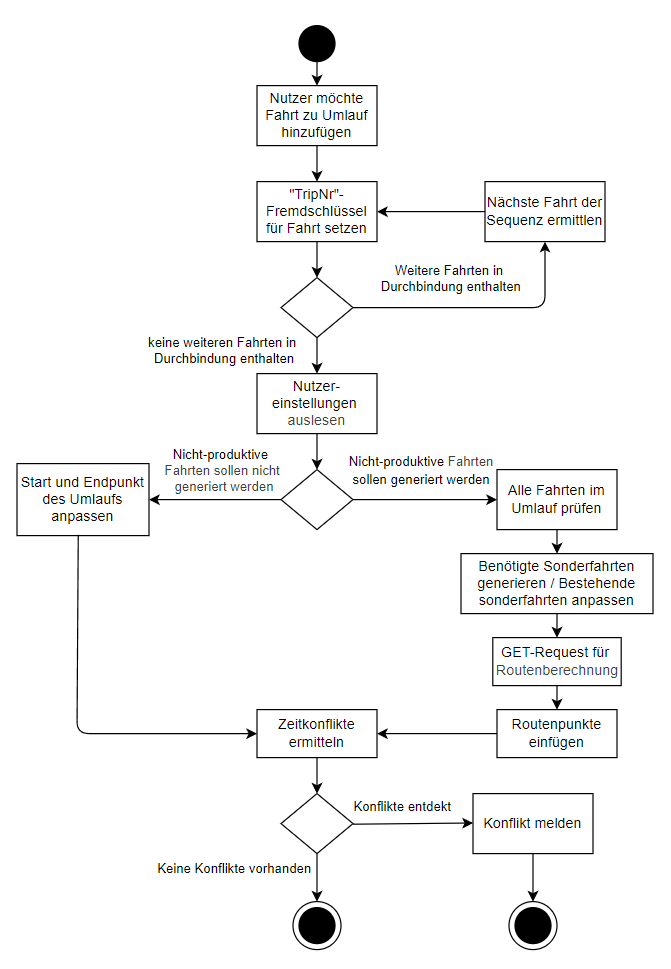
\includegraphics[width=0.8\textwidth]{Ablauf.png}
        \caption{Beziehungen von Umläufen und Fahrten}
        \label{fig:Ablauf}
    \end{figure}

     
\section{"ITCS"}\label{sec:itcs-design}
    Das Projekt \emph{"ITCS"} beinhaltet die SQL-Scripts die alle Änderungen an der Datenbank dokumentierten, um das Schema auf einer neuen Datenbank reproduzieren zu können. 
    Jedem dieser Scripte wird eine aufsteigende Versionsnummer zugeordnet. Diese Versionsnummer wird beim Aufruf des Scripts in eine eigene Datenbanktabelle eingetragen, um den Stand des Schemas
    eindeutig zu dokumentieren. Im Zuge des Praktikums wurde das Datenbank-Schema um einige neuen Tabellen erweitert und bestehende Tabellen um neue Spalten ergänzt. Das resultierte in
    einigen kleineren Create- und Alter-DDL-Scripten. Beispiele dafür sind die Erstellung einer neuen Tabelle für Sonderhaltepunkte oder das Einführen einer neuen Spalte bei Mandanten 
    die abspeichert welche Arten von Sonderfahrten für diese generiert werden sollen.

    Wie bereits erwähnt, liegt der Fokus des Projekts eigentlich auf den Import- und Export-Routinen. Diese werden verwendet, um Daten aus anderen Datenbanken oder Dateien mit dem 
    \emph{VDV-452}~\cite{VDV452} konformen \emph{"x10"}-Format in die ITCS-Datenbank zu importieren. Meist umfasst der Datentransfer eine neue Version des Fahrplans.
    Dieses Projekt nutzt jedoch nicht das \gls{efc} für den Zugriff auf Datenbanken, sondern verwendet die \emph{System.Data.SqlClient}-Bibliothek.
    Diese ist eine .NET-Bibliothek, die es ermöglicht, SQL-Server-Datenbanken zu verwalten 
    und zu manipulieren. Mithilfe dieser wurden ein eigener Datenbaken-Manager und ein attributbasiertes "Object-Relational Mapping" implementiert. Da alle Klassen dadurch von den 
    Basis-Klassen \texttt{Entity} und \texttt{VersionedEntity} erben, ist dieses Vorgehen eher restriktiv, jedoch auf den spezifischen Anwendungsfall optimiert.
    
    Die Routinen für den Import und Export lesen dann Daten aus einer Quelle, speichern diese im Arbeitsspeicher zwischen und schreiben sie dann entweder in eine Datenbank oder in eine Datei.
    Oftmals müssen die Daten dabei angepasst werden, da Quelle und Ziel unterschiedliche Datenschemen verwenden. 

    Der Datenbank-Zugriff und die Routinen wurden jedoch schon vor dem Praktikum implementiert und musste daher nur noch geringfügig angepasst werden, wenn neue Tabellen oder Spalten hinzugefügt wurden.
    Die Anpassungen beschränkten sich dabei auf das Hinzufügen von neuen Methoden im Datenbank-Manager und neuer Domain-Model-Klassen, die die neuen Tabellen repräsentieren.
    
    Im Praktikum wurde dieses Projekt hauptsächlich verwendet, um Methoden, deren Logik in anderen Projekten wiederverwendet werden können sollte, zu implementieren. 
    Dies umfasst beispielsweise die Generierung von Daten wie Metadaten für Sonderfahrten. Wenn die Koordinaten der Sonderhaltepunkte für die neu generierte Sonderfahrt definiert wurden,
    sollte ein \emph{HTTP}-Request an eine externe API gesendet werden, um berechnete Strecke inklusive Fahrtbeschreibung in Form von Wendepunkten zu erhalten. Diese 
    Informationen wird dann aus der \emph{JSON}-Response extrahiert und in der Datenbank gespeichert. Fahrtzeit und -länge werden 
    später für die Ermittlung von Konflikten zwischen Fahrten in Umläufen benötigt. Die Streckenbeschreibung wird für eine 
    visuelle Darstellung der Fahrt benötigt. Diese ist aber nicht mehr Teil des Praktikums.

% \chapter{Das Unternehmen}

% Umfang: 1--2 Seiten
% %%%-----------------------------------------------------------------------------

% \chapter{Projekte und Tätigkeiten während des Praktikums}

% Umfang: 2--3 Seiten (Projektziel(e), Projektumfeld)

% %%%-----------------------------------------------------------------------------
     
% \chapter{Projektbeispiele}

% Umfang: 5--6 Seiten (Umsetzung, grober Terminplan, Ergebnisse,
% Qualitätssicherungsmaßnahmen)

% %%%-----------------------------------------------------------------------------

% \chapter{Erfahrungen und Zusammenfassung}

% Umfang: 1--2 Seiten

%%%-----------------------------------------------------------------------------
\backmatter        % Schlussteil (nur bei Verwendung des Quellenverzeichnisses)
%%%-----------------------------------------------------------------------------

\MakeBibliography % Quellenverzeichnis (sofern notwendig, sonst weglassen)

\end{document}
